%References:
%https://www.quantstart.com/articles/Support-Vector-Machines-A-Guide-for-Beginners#ref-isl
%https://en.wikibooks.org/wiki/Support_Vector_Machines
%http://scikit-learn.org/stable/modules/svm.html
%https://cse.iitk.ac.in/users/piyush/courses/ml_autumn16/771A_lec8_slides.pdf
%http://svmlight.joachims.org/

The chosen model for the discriminative analysis is the \textit{Support Vector Machine} classifier,
an approach for classification that was developed in the computer science community in the 1990s
and that has grown in popularity since then. SVM has been successfully used in many
speech processing fields, such as speaker recognition and pronunciation assessment.
% Podría incluirse alguna mención a que fue el approach discriminativo que usó el paper anterior
% The previous work of the current line proposed
% The baseline work for the current thesis developed

Given a p-dimensional feature space, an SVM \textcolor{red}{(with linear kernel)}
constructs a hyperplane of dimension p - 1
that separates the space in two halves, which allows to classify the instances according
to their relative position to the hyperplane \cite{svm_jwht}. The classification
procedure is then just simply a case of determining which side a test observation falls on.

\textcolor{red}{
If the instances are separable by a hyperplane, then there exists potentially infinite
separating hyperplanes that can be generated from those same instances, because it
is possible to slightly translate or rotate the initial plane without touching any training
observation. Among all of them}, SVM generates the hyperplane that has the largest
distance to the nearest training data points of either of both classes. Such a classifier
is known as Maximal Margin Classifier, and in most of the cases generalizes better to
unobserved data than any of the other possible separating hyperplanes.

One of the key features of the Max Margin Classifier is that the location of the hyperplane
only depends on the support vectors, which are the training observations that lie directly
on the margins' boundaries.

\subsection{Soft Margin} \label{subsection:soft_margin}

One of the problems with Max Margin Classifiers is that they can be very sensitive to the
addition of new training observations: The hyperplane may be adjusted substantially
to force every instance to lie in the right side of the margin or hyerplane, thus leading
to overfitting while reducing the value of the margin (Figure \ref{fig:soft_margin_high_c}).
Moreover, many datasets are not perfectly separable via a linear hyperplane at all.
Because of these reasons, the requirement that a separating hyperplane will perfectly separate
every training observation on the correct side of the line according to its class label can
be relaxed by introducing a new concept developed in \cite{svm_soft_margin}: the Soft Margin.

\begin{figure}[H]
  \centering
  \begin{subfigure}{.5\textwidth}
    \centering
    % 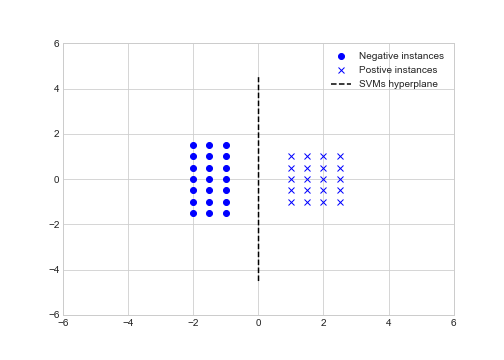
\includegraphics[width=.4\linewidth]{files/figures/method/soft_margin_normal}
    \captionsetup{width=.95\linewidth}
    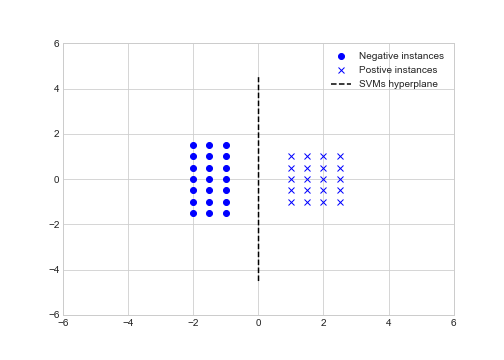
\includegraphics[width=.95\linewidth]{files/figures/method/soft_margin_normal}
    \caption{An initial training set is optimally divided by the Max Margin
    Hyperplane of an SVM}
    \label{fig:sub1}
  \end{subfigure}%
  \begin{subfigure}{.5\textwidth}
    \centering
    \captionsetup{width=.95\linewidth}
    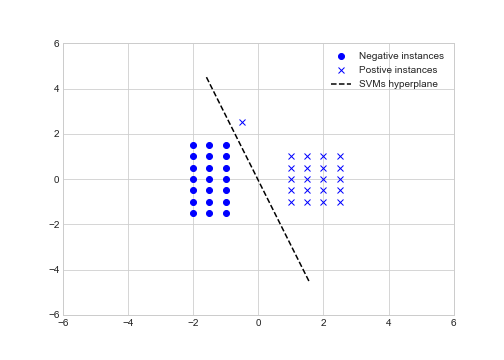
\includegraphics[width=.95\linewidth]{files/figures/method/soft_margin_high_c}
    \caption{The additon of a single instance substantially modifies
    the position of the hyperplane.}
    \label{fig:sub2}
  \end{subfigure}
  \caption{Margin adjustment when inserting a new training instance}
  \label{fig:soft_margin_high_c}
\end{figure}

A Support Vector Classifier or Soft Margin Classifier allows some observations to be on the
incorrect side of the margin or even on the incorrect side of the hyperplane, thus providing
a ``soft'' separation. The soft margin method will choose a hyperplane that splits the example
as cleanly as possible while still maximizing the distance to the nearest training instances.
The effects of the soft margin can be observed in Fig. \ref{fig:soft_margin_low_c}.

Given a labeled dataset D of $n$ points
of the form: $D=\{ \ (x_{i}, y_{i}) \ | \ x_{i} \in R^{p}, \ y_{i} \in \{-1, 1\} \ \}$, the
problem can be formulated as:

% \begin{equation}
%   \displaystyle \min_{\omega, \xi} \left\{ \frac{1}{2}{\| w \|}^{2} + C \sum_{i=i}^{n}\xi_{i} \right\}
% \end{equation}

% Subject to (for any $i = 1 \ldots n$):

% \begin{equation}
%   y_{i}*(\omega^{t} \cdot x_{i} + b \ ) \geq 1 - \xi_{i}, \ \xi_{i} \geq 0
% \end{equation}

\textcolor{red}{
  \begin{equation}
  % \begin{align}
    \displaystyle \min_{\omega, \xi} \left\{ \frac{1}{2}{\| w \|}^{2} + C \sum_{i=i}^{n}\xi_{i} \right\}, \ s.t \ \forall i: \
    y_{i}*(\omega^{t} \cdot x_{i} + b \ ) \geq 1 - \xi_{i}, \ \xi_{i} \geq 0
  % \end{align}
  \end{equation}
}

Each $x_{i}$ is a p-dimensional real number vector.
The hyperplane $\omega^{t} \cdot x + b = 0$ splits the \textcolor{red}{space in two halves}.
The condition $y_{i}*(\omega^{t} \cdot x_{i} - b) \geq 1$ for any instance $x_{i}$ is
known as the margin condition,
\textcolor{red}{
  and ensures a margin $\gamma$ on each side of at least
  $\frac{1}{\| \omega \|}$:
}

\begin{equation}
  \gamma = \frac{ |\omega^{t} \cdot x_{i} + b| }{ \| \omega \| } \geq \frac{1}{\| \omega \|}
\end{equation}

Finally, slack variables $\xi_{i}$ allow the individual observations to be
on the wrong side of the
margin or hyperplane, while $C$ is an input parameter that determines the cost of
the errors, thus establishing a trade off between a large margin and the error penalty.

\begin{figure}[H]
  \centering
  % \captionsetup{width=.95\linewidth}
  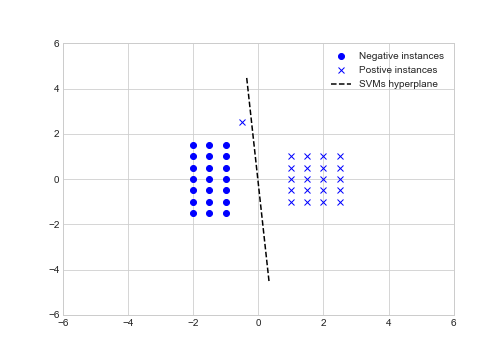
\includegraphics[width=.55\linewidth]{files/figures/method/soft_margin_low_c}
  \caption{When lowering the cost of misclassifications ($C$ parameter), the SVM still
  prioritizes maximizing the margin, allowing an instance to end in the wrong side
  of the hyperplane.}
  \label{fig:soft_margin_low_c}
\end{figure}

To conclude this section, it is worth mentioning that feature scaling is an important
step to be performed before training
the linear SVM classifier to avoid the \textcolor{red}{dominance} of the
features with highest values
when calculating the hyperplane. For this reason both supervectors
and dynamic features are standardized by removing the mean and scaling to unit variance
before training.

% [avg. x*x]^-1

% \subsection{SVM initial version}

% The SVM is a member of the family of
% \textit{maximal margin classifiers}, which base its strategy in finding the hyperplane that
% best separate the positive and negative instances \cite{svm_jwht}.

% \subsection{Maximal Margin Classifiers}
% In a \textit{p-dimensional} space, a hyperplane is a flat affine subspace of
% dimension $p-1$ defined by the equation:

% \begin{equation}
%   \label{eq:hyperplane}
%   \beta_{0} + \beta_{1}X_{1} + \beta_{2}X_{2} + \dotsc + \beta_{p}X_{p} = 0
% \end{equation}

% The equation defines a \textit{p-dimensional} hyperplane in the sense that if a point
% $X=(X_{1}, X_{2}, \dotsc, X_{p})^{T}$ in \textit{p-dimensional} space
% satisfies \ref{eq:hyperplane} then $X$ lies on the hyperplane.

% If $X$ doesn't lie in the hyperplane then either:

% \begin{equation}
%   \label{eq:hyperplaneGreater}
%   \beta_{0} + \beta_{1}X_{1} + \beta_{2}X_{2} + \dotsc + \beta_{p}X_{p} > 0
% \end{equation}

% \begin{center}or\end{center}

% \begin{equation}
%   \label{eq:hyperplaneLesser}
%   \beta_{0} + \beta_{1}X_{1} + \beta_{2}X_{2} + \dotsc + \beta_{p}X_{p} < 0
% \end{equation}

% So the hyperplane somehow divides the \textit{p-dimensional} space into two halves. One can
% easily determine on which side of the hyperplane a point lies by simply calculating the sign
% of the left hand side of \ref{eq:hyperplane}.

% Having a set of $n$ instances of dimension $p$, with labels
% $y_{1}, y_{2}, \dotsc y_{n} \in \{-1,1\}$ and $x^{i} = (x^{i}_{1}, x^{i}_{2}, \dotsc x^{i}_{p}) \ \forall \ 1 \leq i \leq {n}$ and supposing that it is possible to construct a hyperplane that
% separates the training observations perfectly according to their class labels, then a
% separating hyperplane has the property that:

% \begin{equation}
% \beta_{0} + \beta_{1}X_{1} + \beta_{2}X_{2} + \dotsc + \beta_{p}X_{p} > 0 \ if \ y_{i} = 1
% \end{equation}

% \begin{center}and\end{center}

% \begin{equation}
% \beta_{0} + \beta_{1}X_{1} + \beta_{2}X_{2} + \dotsc + \beta_{p}X_{p} < 0 \ if \ y_{i} = -1
% \end{equation}

% A test observation $x^{*}$ is classified based on the sign of
% $f(x^{*})=\beta_{0}+\beta_{1}x^{*}_{1} + \beta_{2}x^{*}_{2} + \dotsc + \beta_{p}x^{*}_{p}$.
% If $f(x^{*})$ is positive, then it is assigned to class 1 whereas if $f(x^{*})$ is negative
% then it is assigned to class -1. In addition, the magnitude of $f(x^{*})$ also contains valuable
% information.
% If $f(x^{*})$ is far from zero then it means that $x^{*}$ lies far from the hyperplane
% whereas if $f(x^{*})$ is close to zero then $x^{*}$ is located near the hyperplane and
% there is less certainty about the class of $x^{*}$.

% In general, if the data can be perfectly separated using a hyperplane, then there will be an
% infinite number of such hyperplanes. This is because a given separating hyperplane can usually
% be shift a tiny bit up or down, or rotating without coming into contact with any of the
% observations.

% \begin{figure}[H]
%   \centering
%   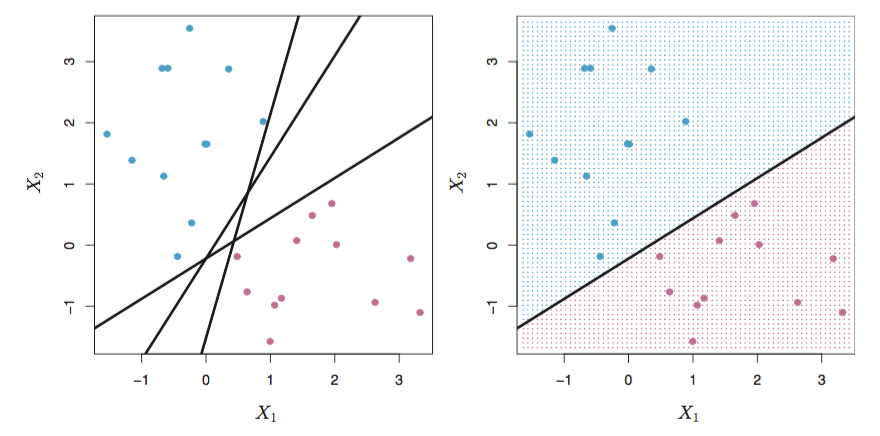
\includegraphics[width=0.8\textwidth]{files/figures/method/max-margin}
%   \caption{Taken from \textit{JWHT} \cite{svm_jwht} book.
%   Left: Three separating hyperplanes out of many
%   possibilities. Right: Optimal Separating Hyperplane for the same dataset. A test observation
%   that falls in the blue portion of the grid will be assigned to the blue class, and a test
%   observation that falls in the purple portion of the grid will be assigned
%   to the purple class.}
%   \label{fig:maxMargin}
% \end{figure}

% A natural choice is the \textit{Maximal Margin Classifiers} (also known as the
% \textit{Optimal Separating Hyerplane}), which is the separating hyperplane that is farthest
% from the training observations. The \textit{margin} of the hyperplane is computed as the
% minimal perpendicular distance to the hyperplane among all the training observations.
% The maximal margin hyperplane is the separating hyperplane for which the margin is the largest.
% The core idea is that a classifier that has a large margin on the training data will also
% have a large margin on the test data.

% \subsection{Support Vectors}

% The separating hyperplane is determined by the instances of both classes that lies on the margin
% of the hyperplane. These observations are known as \textit{Support Vectors}.
% Observations can be interpreted as vectors in a \textit{p-dimensional} space and they
% "support" the maximal
% margin hyperplane in the sense that if these points were moved slightly then the maximal
% margin hyperplane would move as well. The maximal margin hyperplane depends directly on the
% support vectors, but not on the other observations: a movement to any of the other observations
% would not affect the separating hyperplane, provided that the observation's movement does not cause
% it to cross the boundary set by the margin.

% \begin{figure}[H]
%   \centering
%   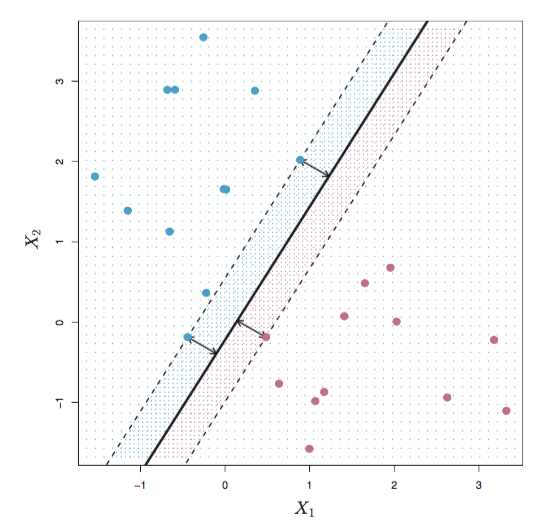
\includegraphics[width=0.4\textwidth]{files/figures/method/support-vectors}
%   \caption{Taken from \textit{JWHT} \cite{svm_jwht} book. The maximal margin hyperplane
%   is shown as a solid line. The margin is the distance between the solid line to either
%   of the dashed lines. The two blue points and the purple point that line on the
%   dashed lines are the support vectors.}
%   \label{fig:maxMargin}
% \end{figure}

% \subsection{Problem Formulation}

% It can be proven that given a set of $n$ observations of dimension $p$, the problem of
% finding the \textit{Maximal Margin Hyperplane} can be posed as an optimization problem.
% The perpendicular distance from the observation $x^{*}$ is determined by the equation:
% % In order to
% % minimize $\| w \| = (\beta_{1}, \dotsc, \beta_{p})$.

% \begin{equation}
% \label{eq:svmOptimization}
% \frac{w^{T}x^{*}}{\| w \|} = p \implies w^{T}x^{*} = p{\| w \|}
% \end{equation}

% $p$ is the length of the projection of the observation $x^{*}$
% onto the normal vector of the hyperplane, i.e, the distance to the hyperplane.
% Equation \ref{eq:svmOptimization} states that in order to maximize $p$ the norm of $w$
% has to be minimized. On the other hand, the minimization problem is subject to the constraint:

% \begin{equation}
%   \label{eq:svmConstraint}
%   y_{i} * (\beta_{0} + \beta_{1}x_{1} + \beta_{2}x_{2} + \dotsc + \beta_{p}x_{p}) > 0 \ \forall \ 1 \leq i \leq {n}
% \end{equation}

% Equation \ref{eq:svmConstraint} can be easily derived from \ref{eq:hyperplaneGreater} and
% \ref{eq:hyperplaneLesser}.  This context matches the necessary conditions to apply
% the \textit{Lagrange Multipliers} technique, to get this problem into a form
% that can be solved analytically.

% In practice, real data is scarcely ever completely linearly separable
% and there is a trade off between
% minimizing $\| w \|$ (i.e separating the instances by the largest possible margin)
% and satisfying the constraint imposed over every
% observation to lie on the right side of the hyperplane.
% The desired hyperplane is one which separates correctly the vast majority of the observations and
% at the same time it separates them by the largest margin. For this reason, when training an
% \textit{SVM} classifier an additional parameter $C$ is passed as argument to the training
% method in order to prioritize one problem over the other. A bigger $C$ favors the correctly
% classification of the instances, while a smaller one favors the minimization of $\| w \|$
% and thus finding the hyperplane with the largest margin for most of the instances, allowing
% some instances to be on the wrong side of the margin and even on the wrong side of the
% hyperplane.

% \begin{figure}[H]
%   \centering
%   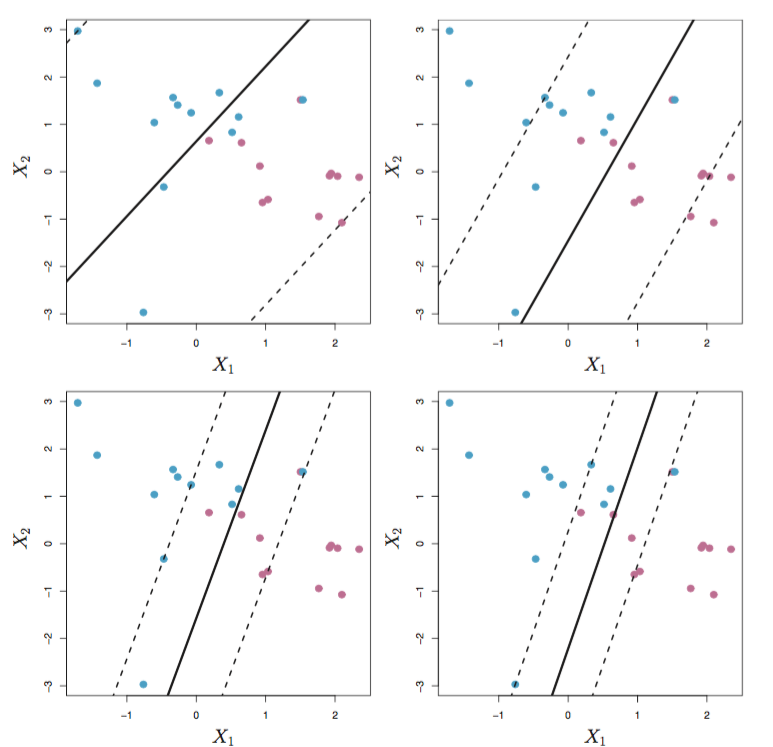
\includegraphics[width=0.7\textwidth]{files/figures/method/c-effects}
%   \caption{Taken from \textit{JWHT} \cite{svm_jwht} book. Different effects in an SVM
%   when varying $C$ value. The smallest value of $C$ is used in the top left,
%   following an increasing order from left to right and top to bottom. When $C$ is small,
%   then there is a high tolerance for observations being on the wrong side of the margin,
%   and so the margin will be large. As $C$ increases, the tolerance for observations
%   being on the wrong side of the margin decreases, and the margin narrows.}
%   \label{fig:maxMargin}
% \end{figure}

% Finally, it is worth mentioning that in some cases an effective classification of the
% observations of a given dataset may require a non-linear decision boundary. For that cases,
% \textit{SVM} classifiers relies on special functions called \textit{kernels} that transform
% the feature space into a space that can be linearly separable. The current work assumes
% that the input features are linearly separable and therefore uses a linear kernel,
% so there is no need to analyse kernels in detail.
% However, for other experiments involving
% different data an \textit{SVM} classifier may require different types of kernels
% such as \textit{polynomial} or \textit{radial} kernels.